% =============================================
% =============================================
% Document class: Article
\documentclass[ a4paper, twoside, 11pt]{article}
% Packages: LaTeX (Depth-1)
\usepackage[ vlined, linesnumbered, ruled]{algorithm2e}
\usepackage{ amsfonts, amsmath, amssymb, amsthm}
\usepackage[ titletoc, title]{appendix}
\usepackage{ bbm}
\usepackage{ color}
\usepackage{ dsfont}
\usepackage{ enumitem}
\usepackage{ graphicx}
\usepackage{ fancyhdr, float, fullpage}
\usepackage{ hyperref}
\usepackage{ lastpage, latexsym, lipsum}
\usepackage{ mathrsfs, mathtools, multicol}
\usepackage{ parskip}
\usepackage{ setspace, stmaryrd, subcaption}
\usepackage{ tabularx}
\usepackage{ wasysym}
\usepackage[ dvipsnames, table]{ xcolor}
\usepackage{ xfrac}
% Packages: LaTeX (Depth-2)
\usepackage{ epstopdf}

% =============================================
\topmargin 			= -1.6cm
\headheight 		= .90cm
\headsep 			= .80cm
\textheight 		= 24.0cm
\textwidth 			= 15.5cm
\oddsidemargin		= 0.cm
\evensidemargin 	= 0.cm

% =============================================
% =============================================
% Macros: Language
\newcommand{\define}{\triangleq}
\newcommand{\done}{\hfill $\square$}
%\newcommand{\eqCIRC}{\stackrel{\circ}{=}}
%\newcommand{\eqSTAR}{\stackrel{*}{=}}
\renewcommand{\epsilon}{\varepsilon}
\newcommand{\eg}{\textit{e.g.,\;}}
\newcommand{\egc}{\textit{e.g.:\;}}
\newcommand{\Eg}{\textit{E.g.,\;}}
\newcommand{\Egc}{\textit{E.g.:\;}}
\newcommand{\ie}{\textit{i.e.,\;}}
\newcommand{\iec}{\textit{i.e.:\;}}
\newcommand{\Ie}{\textit{I.e.,\;}}
\newcommand{\Iec}{\textit{I.e.:\;}}
\newcommand{\QED}{\hfill $\blacksquare$}
\renewcommand{\tilde}[1]{\widetilde{#1}}
\newcommand{\tsup}[1]{\ensuremath{^{\text{#1}}}}
\newcommand{\tsub}[1]{\ensuremath{_{\text{#1}}}}
\renewcommand{\vec}[1]{{\boldsymbol{#1}}}

% Macros: Optimization & Probability
\DeclareMathOperator*{\argmax}{arg\,max}
\DeclareMathOperator*{\argmin}{arg\,min}
\newcommand{\Exp}{\mathbb{E}}
\newcommand{\Indicate}[1]{ \IndFun \, \{ \, #1 \, \} }
\renewcommand{\Pr}{\mathbb{P}}
\newcommand{\Normal}{\mathcal{N}}
\newcommand{\std}{\text{std}}
\newcommand{\var}{\text{var}}

% Macros: Sets
\newcommand{\Complex}{\mathbb{C}}
\renewcommand{\emptyset}{\varnothing}
\newcommand{\Nat}{\mathbb{N}}
\renewcommand{\Re}{\mathbb{R}}
\newcommand{\ReNN}{{\Re}_{\geq 0}}
\newcommand{\ReSP}{{\Re}_{> 0}}
\renewcommand{\subset}{\subseteq}
\renewcommand{\supset}{\supseteq}
\newcommand{\Z}{\mathbb{Z}}
\newcommand{\ZNN}{{\Z}_{\geq 0}}

% Macros: Spacing & Other Commands
\newcommand{\fullcut}{\vspace{-\baselineskip}}
\newcommand{\fullskip}{\vspace{\baselineskip}}
\newcommand{\halfcut}{\vspace{-0.5\baselineskip}}
\newcommand{\halfskip}{\vspace{0.5\baselineskip}}
\renewcommand{\figurename}{Figura}
\renewcommand{\tablename}{Tabla}

% =============================================
% Sesion de Clase
\newcommand{\sesion}{06}
% Macros para definiciones, teoremas, etc
\newcounter{sesion}
\setcounter{sesion}{\sesion}
\theoremstyle{definition}
\newtheorem{definition}{Definici\'on}[sesion]
\newtheorem{example}[definition]{Ejemplo}
\newtheorem{exercise}[definition]{Ejercicio}
\newtheorem{note}[definition]{Nota}
\newtheorem{problem}[definition]{Problema}
\newtheorem{theorem}[definition]{Teorema}

% =============================================
% =============================================
\newcommand{\HeaderLine}{}
\newcommand{\FooterLine}{P\'agina \thepage ~de \pageref*{LastPage}}

\pagestyle{fancyplain}
\fancyhf{}

\rhead[]{\fancyplain{}{\HeaderLine}}
\lhead[\fancyplain{}{\HeaderLine}]{}
\lfoot[\fancyplain{}{\FooterLine}]{}
\rfoot[]{\fancyplain{}{\FooterLine}}

\renewcommand{\headrulewidth}{0.4pt}
\renewcommand{\footrulewidth}{0.4pt}
\renewcommand{\thefootnote}{\fnsymbol{footnote}}

% =============================================
% =============================================
\begin{document}
\allowdisplaybreaks

\begin{center}
\Large Din\'amica (FIMCP-01271): Lecci\'on \sesion \\[0.5ex]
\small \textbf{A\~no:} 2016-2017 \qquad \textbf{T\'ermino:} II \qquad
\textbf{Instructor:} Luis I. Reyes Castro \qquad \textbf{Paralelo:} 02
\end{center}
\halfskip

\fbox{

\begin{minipage}[b][\height][t]{\textwidth}
\vspace{0.2 cm}

\begin{center}
\textbf{COMPROMISO DE HONOR}
\end{center}
\vspace{0.4 cm}

\scriptsize
{
Yo, \rule{60mm}{.1pt} al firmar este compromiso, reconozco que la presente lecci\'on est\'a dise\~nada para ser resuelta de manera individual, que puedo usar un l\'apiz o pluma y una calculadora cient\'ifica, \linebreak que solo puedo comunicarme con la persona responsable de la recepci\'on de la lecci\'on, y que cualquier instrumento de comunicaci\'on que hubiere tra\'ido debo apagarlo. Tambi\'en estoy conciente que no debo consultar libros, notas, \linebreak ni materiales did\'acticos adicionales a los que el instructor entregue durante la lecci\'on o autorice a utilizar. Finalmente, me comprometo a desarrollar y presentar mis respuestas de manera clara y ordenada. \\

Firmo al pie del presente compromiso como constancia de haberlo le\'ido y aceptado. 
\vspace{0.4 cm}

Firma: \rule{60mm}{.1pt} \qquad N\'umero de matr\'icula: \rule{40mm}{.1pt} \hspace{0.5cm} \\[-0.8ex]

}

\end{minipage}

}
\fullskip

% =============================================
\begin{problem}
\textbf{[10 Puntos]} El cuerpo $AB$ y la barra $BC$ del componente rob\'otico que se muestra en la figura giran a la raz\'on constante $\omega_1 = 0.60$ rad/s alrededor del eje $Y$. \linebreak De manera simult\'anea un control de alambre y polea ocasiona que el brazo CD gire alrededor de $C$ a raz\'on constante $\omega_2 = d\beta / dt = 0.45$ rad/s. En el instante mostrado, cuando $\beta = 120^{\circ}$, determine: 
\begin{itemize}
\item La velocidad angular de la barra $CD$. 
\item La aceleraci\'on angular de la barra $CD$. 
\item La velocidad del punto $D$. 
\item La aceleraci\'on del punto $D$. 
\end{itemize}

\begin{figure}[htb]
\centering
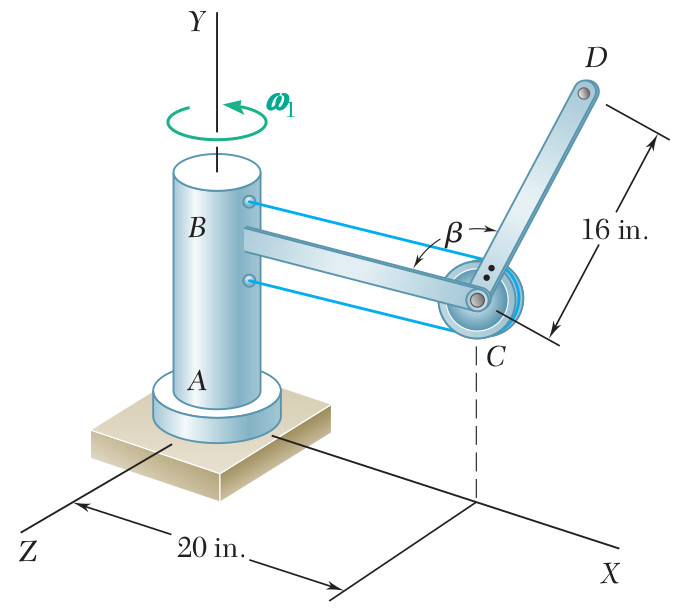
\includegraphics[ width = 0.5\textwidth]{fig_P15-234.jpg}
\end{figure}

\emph{Sugerencia:} Existen al menos dos maneras de resolver este problema. Una es escribir la velocidad angular de la barra $CD$ como funci\'on del tiempo y diferenciar dicha expresi\'on para hallar la aceleraci\'on angular. La otra es usar marcos de referencia rotatorios. 

\end{problem}
\vspace{\baselineskip}

% =============================================
\begin{problem}
\textbf{[10 Puntos]} 
La barra $AB$ de 25 in de longitud se conecta mediante uni\'on de r\'otula a los collarines $A$ y $B$, los cuales se deslizan a lo largo de las dos barras en la forma que se indica. En el instante mostrado, el collar\'in $B$ se mueve hacia el soporte $E$ a una rapidez constante de 20 in/s. Con esto en mente, escriba un conjunto de cuatro ecuaciones lineales de cuya soluci\'on se pueda encontrar la velocidad del collar\'in $A$, denotada $\vec{v_A} = v_A \, \vec{\hat{j}}$, y la velocidad angular de la barra $AB$, denotada $\vec{\omega} = ( \, \omega_x, \, \omega_y, \, \omega_z)$, en el instante mostrado. (Dichas ecuaciones quedar\'an expresadas en t\'erminos de las inc\'ognitas $v_A$, $\omega_x$, $\omega_y$ y $\omega_z$.) 

\begin{figure}[htb]
\centering
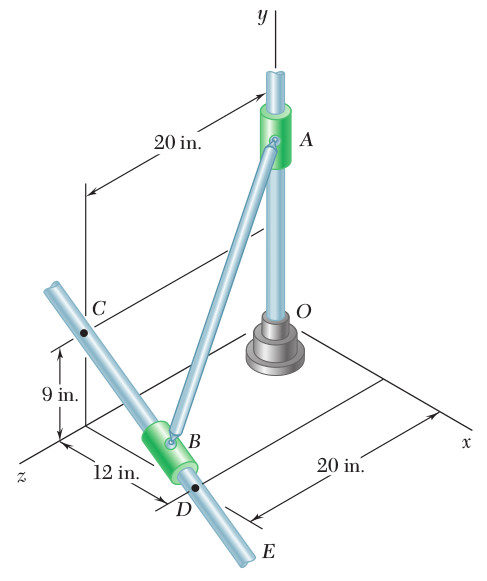
\includegraphics[ width = 0.54\textwidth]{fig_prob_barra.jpg}
\end{figure}

\end{problem}
\vspace{\baselineskip}

\end{document}
